% 加密算法实例程序的编译运行与测试
\subsection{SM4示例程序的测试使用}
按照实验指导书的指示分别安装依赖、获取libboundscheck源码并编译、获取openhitls源码并编译、
然后运行实例代码,结果如下图:
\begin{figure}[H]
    \centering
    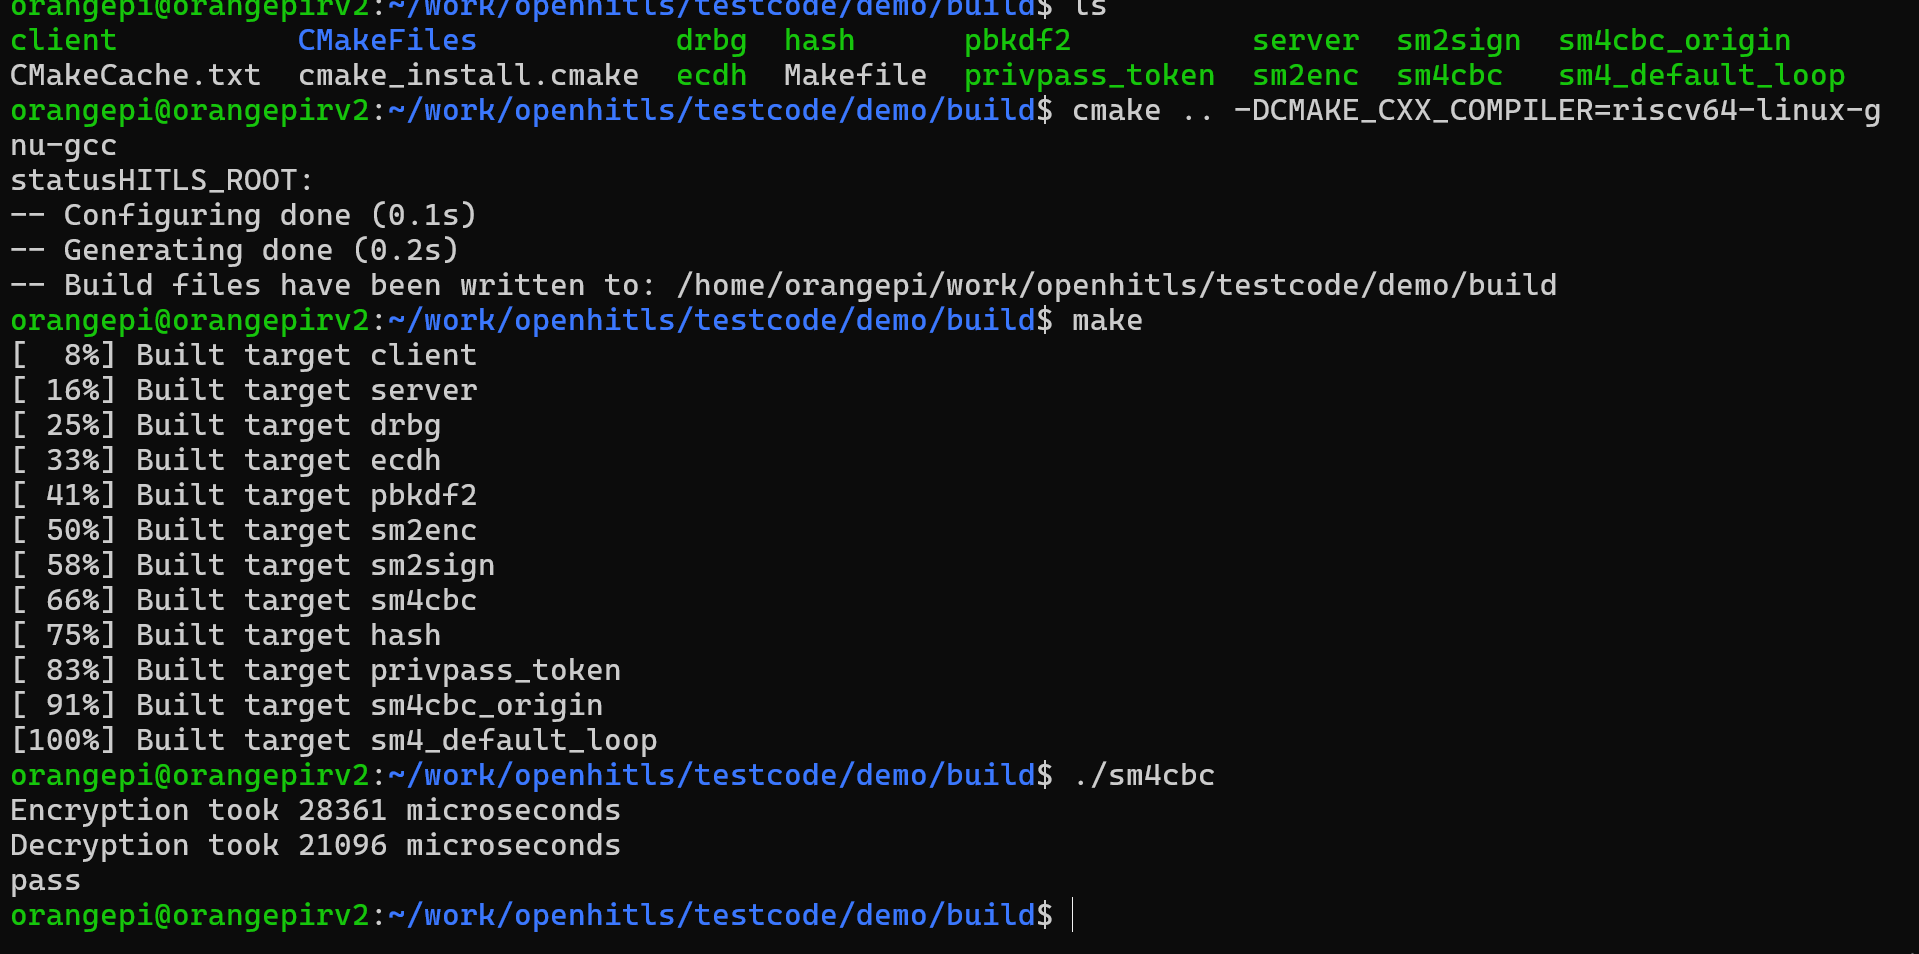
\includegraphics[width = 0.9\textwidth]{figure/sm4encrypt_example.png}
    \caption{SM4示例程序测试运行}
\end{figure}

\subsection{SM3示例程序的使用测试}
修改hash.c文件中的部分代码,重新编译即可测试运行SM3示例程序,结果如下:
\begin{figure}[H]
    \centering
    \begin{minipage}{0.49\linewidth}
        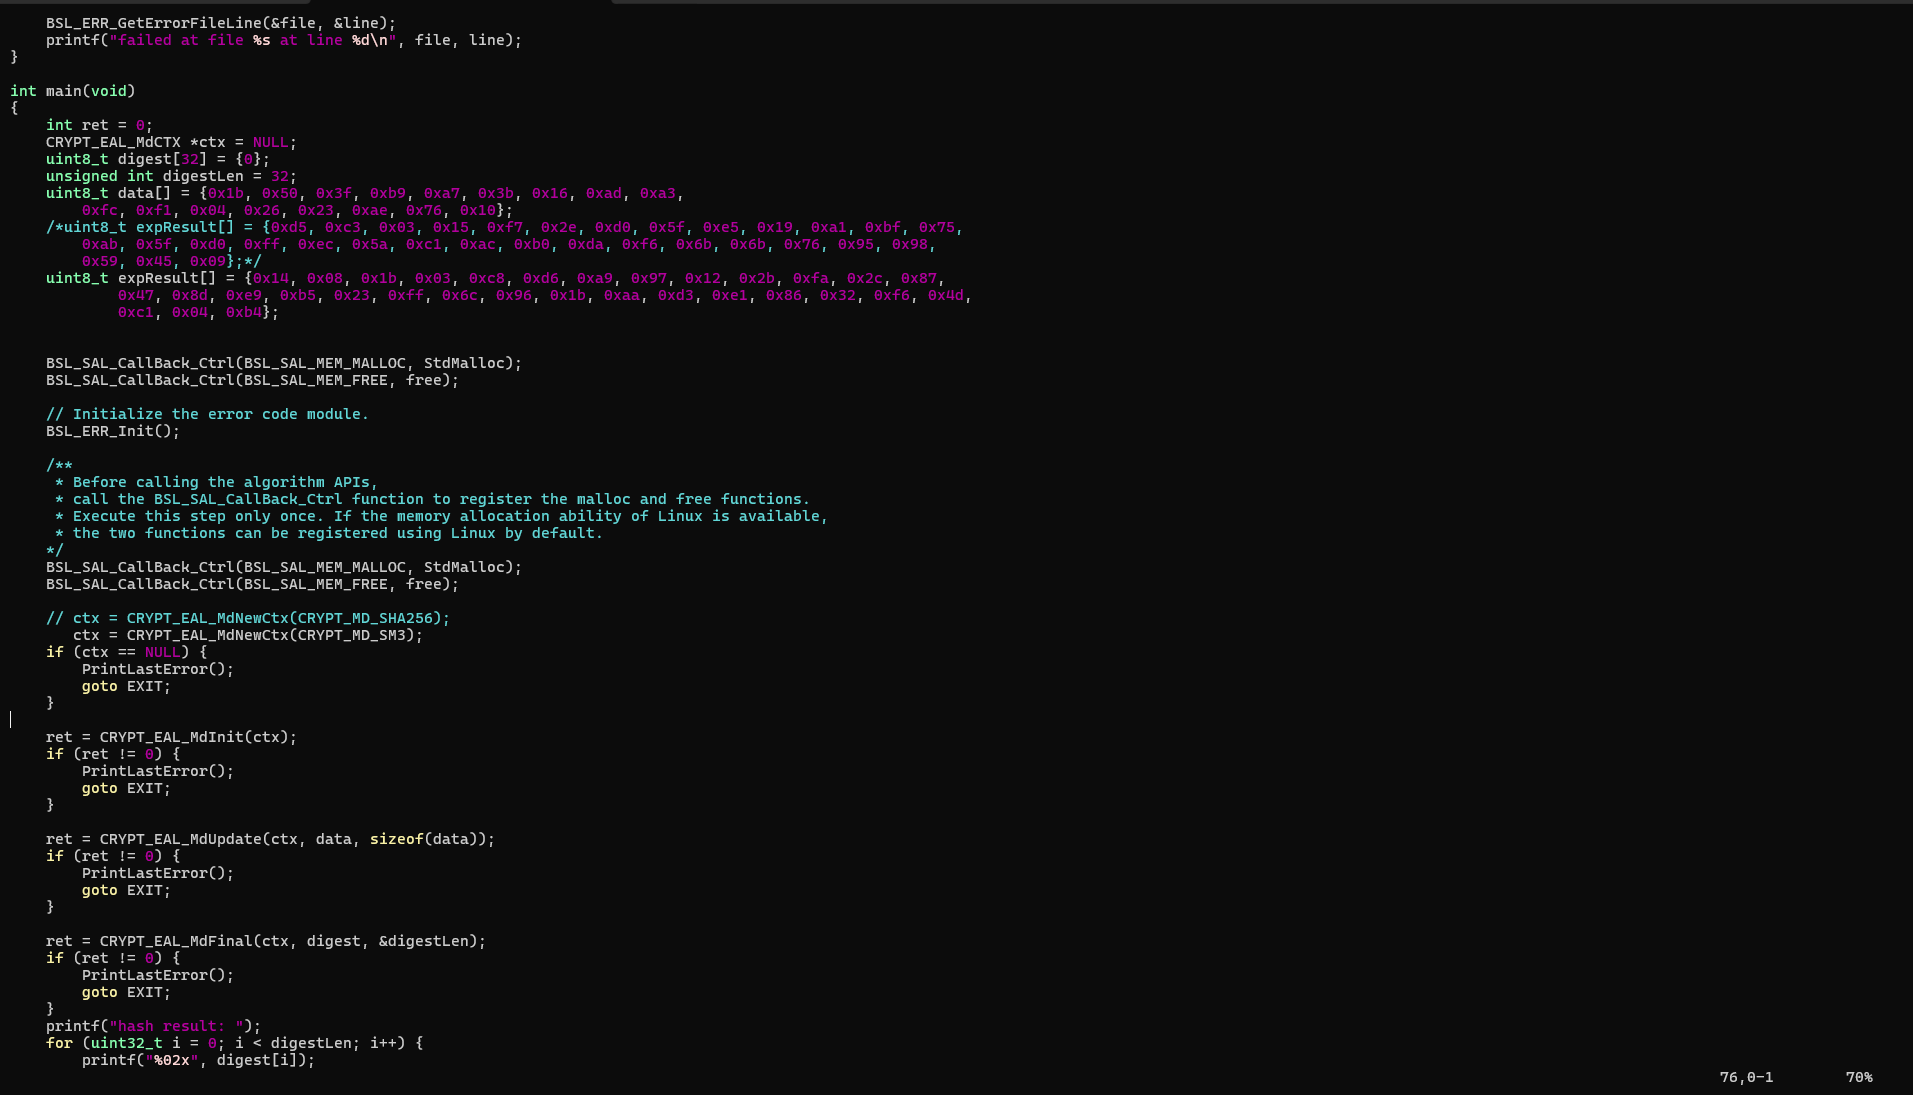
\includegraphics[width = 1\textwidth]{figure/change_code_sm3.png}
        \caption{修改代码}
    \end{minipage}
    \begin{minipage}{0.49\linewidth}
        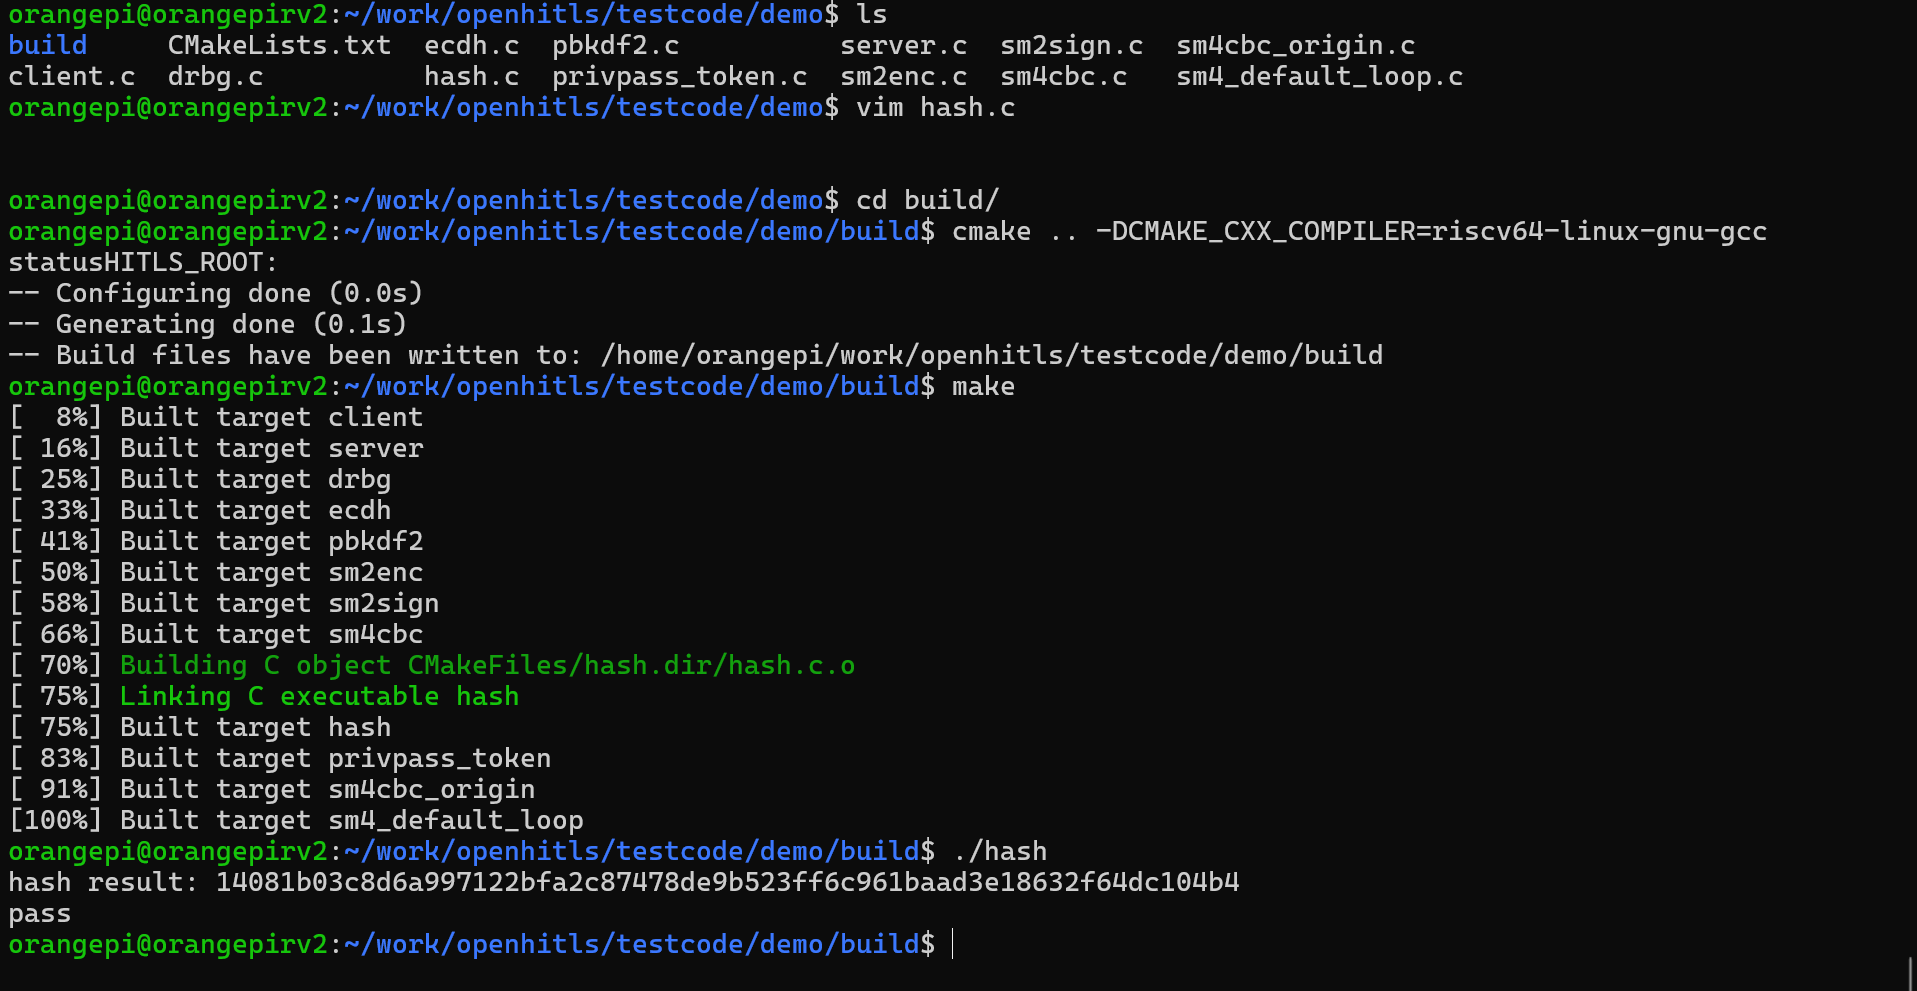
\includegraphics[width = 1\textwidth]{figure/sm3_example.png}
        \caption{sm3示例程序测试运行}
    \end{minipage}
\end{figure}



